The Uhuru X-ray Explorer Satellite launched in 1970 provided the first evidence of galaxy cluster X-ray emission. It showed that high mass galaxy clusters can emit high-energy light. A few years later, the Einstein Observatory was able to also detect the X-ray spectrum of smaller clusters. Moreover, it showed that the X-ray source is more homogeniously spread within the galaxy cluster and not bound to single galaxies. This indicates that the intercluster medium (ICM) consists of gas which is heated to several tens of millions of Kelvin. In this plasma, free electrons create radiaton by moving through the coulomb potential of an atom. This so called bremsstrahlung, or free-free radiation in the case of a plasma, generates the observed X-ray spectrum. 

\begin{figure}[h]
 \centering
 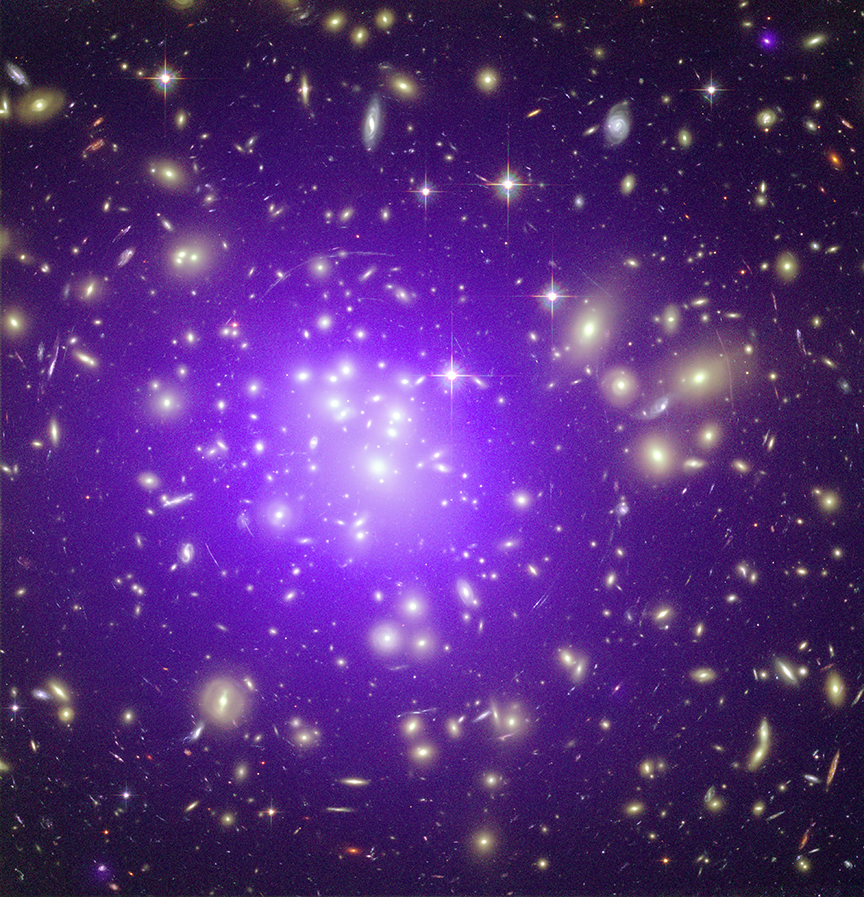
\includegraphics[width=0.5\textwidth]{images/Chapter2/a1689.jpg}
 \caption{Composite image of the galaxy cluster Abell 1689. Visible light is shown in yellow and X-ray in violet \citep{hubble-2010}}
 \label{fig:Abell1689}
\end{figure}

To investigate the X-ray spectrum of a galaxy cluster consider \eqref{emiss}:

\begin{equation}
\label{emiss}
    \epsilon^{ff}_{\nu} = \frac{32\pi Z^2 e^6 n_e n_i}{3m_ec^3}\sqrt{\frac{2\pi}{3k_B T m_e}}e^{-hp\nu/k_B T}g_{ff}(T,\nu)
\end{equation}

\begin{equation}
\label{emiss_g}
g_{ff} \approx \frac{3}{\sqrt{\pi}}\ln{\frac{9k_B T}{4h_P \nu}} \approx 1
\end{equation}

$\epsilon^{ff}_{\nu}$ is the emissivity of the bremsstrahlung where Z is the charge of the ions, $e$ the elemental charge, $n_e$ and $n_i$ the electron and ion density, $h_P \nu$ the photon energy, $k_BT$ the thermal energy, $m_e$ the electron mass, $c$ the speed of light and $g_{ff}$ the Gaunt factor which takes quantum mechanical effects into account. For classical problems $g_{ff}$ is set to $1$.

Using this equation, one finds a flat continuity region for $h_p \nu \ll k_B T$. This continuity region is cut off exponentially for higher energies ($h_p \nu > k_B T$). Photoabsoption cuts off the lowest energy part of the continuity region giving us the spectrum in \autoref{fig:x-ray_emission_curves}

\begin{figure}[h]
 \centering
 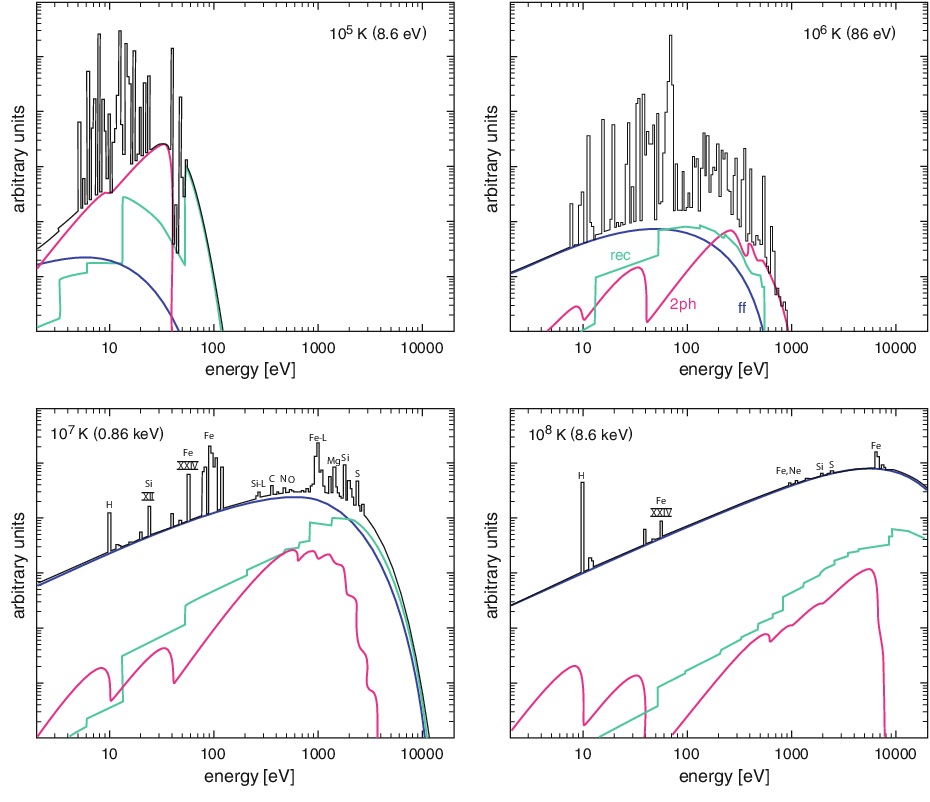
\includegraphics[width=1\textwidth]{images/Chapter2/9-Figure6-1.png}
 \caption{Free free radiation at different plasma temperatures including photo absorption (blue). Recombination radiaton (green) and two-photon radiation (red) are shown for comparison of the dominating source of radiation. Absorption and emission lines are shown in black.  \citep{Boehringer2010}}
 \label{fig:x-ray_emission_curves}
\end{figure}

In the case of galaxy clusters, we have temperatures $> 10^6K$ making the X-ray radiation the spectrum's dominant part. Emission lines become more disruptive at lower temperatures whilst at $T > 10^7K$ especially the emission from iron and silicon are most notable.

Using this relation between the X-ray spectrum and the plasma temperature, it is possible to estimate cluster temperatures. Moreover, it is possible to use this knowledge to work out scaling relations to estimate galaxy cluster masses (see \cref{mass_est}).